\question{2,0}~Especifique um relógio que se ``preocupa'' somente em
mostrar as horas no padrão 24 horas.

\question{2,5}~Especifique um relógio que se ``preocupa'' em mostrar as horas e
minutos, também no padrão 24 horas.

\question{2,0}~Faça a especificação de um sistema de transferência de dinheiro
entre conta corrente e poupança, onde a conta corrente não pode ter saldo negativo. Lembrando
que o dinheiro deve ser subtraído primeiro da conta corrente e depois adicionado
na conta poupança. Explique o problema que pode ocorrer de não se controlar esta
sequência. Adicione as invariantes que achar necessárias.
\exercise~Especifique um relógio que se ``preocupa'' somente em mostrar as
horas no padrão 12 horas.

\exercise~Especifique um relógio que se ``preocupa'' em mostrar as horas e
minutos, também no padrão 12 horas.

\exercise~Faça a especificação de um sistema de transferência de dinheiro
entre 2 contas (A e B) em que nenhuma das duas pode ter saldo negativo. Lembrando
que o dinheiro deve ser subtraído primeiro da conta de origem e depois adicionado
na conta destino. Explique o problema que pode ocorrer de não se controlar esta
sequência. Adicione as invariantes que achar necessárias. 

\exercise~Foi requisitado um sistema para controle de um experimento
de caracterização de material, que consiste em colocar a peça do
material que se deseja caracterizar em um recipiente com uma
resistência acoplada e aquecê-lo até a temperatura de 120 graus
Celsius. Ao atingir esta temperatura, é feito o resfriamento com a
adição de nitrogênio líquido no compartimento, até atingir a
temperatura de 20 graus Celsius, onde é feito o aquecimento de novo
até 120 graus e resfriado de novo até 20 graus, sendo que após atingir
este ponto o experimento é encerrado. Especifique o sistema usando
TLA$^+$.

% fonte: https://quimicacidentes.wordpress.com/2017/10/22/a-maquina-therac/
\exercise~A máquina Therac-25 era uma máquina de radioterapia
controlada por computador, a máquina trabalhava com dois tipos de
tratamento:

\begin{itemize}
\item Terapia de feixe de elétrons direto: aplicava desde baixas energias
 até energias altas em um curto período de tempo.

\item Terapia com raio X: usava o feixe de elétrons de 25MeV, passando
por um alvo ({\em target}) de tungstênio que convertia os elétrons em
raios X.

Os acidentes ocorriam quando o feixe de alta intensidade era ativado
sem o alvo ({\em target}) ter sido posicionado para seu lugar
(Figura~\ref{fig:therac}).
\end{itemize}

\begin{figure}\centering
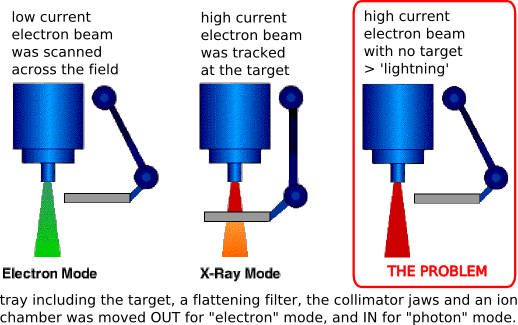
\includegraphics[scale=.4]{therac25.png}
\caption{Ilustração do acidente ocorrido devido ao erro no software da máquina Therac-25.}
\label{fig:therac}
\end{figure}

Com base nessas informações, faça uma especificação em TLA$^+$ de um
módulo de sistema que poderia evitar que o feixe de alta intensidade
fosse ativado sem o alvo ({\em target}).